% VUT FIT MITAI
% PRL 2019/2020
% Project 3: Viditelnost
% Author: Vladimir Dusek
% Login: xdusek27

%%%%%%%%%%%%%%%%%%%%%%%%%%%%%%%%%%%%%%%%%%%%%%%%%%%%%%%%%%%%%%%%%%%%%

\documentclass[11pt, a4paper, titlepage]{article}
\usepackage[left=2cm, text={17cm, 24cm}, top=3cm]{geometry}
\usepackage[utf8]{inputenc}
\usepackage[czech]{babel}
\usepackage{pdfpages}
\usepackage[T1]{fontenc}
\usepackage{amsfonts}
\usepackage{float}

% \setlength\parindent{0pt}

\begin{document}

%%%%%%%%%%%%%%%%%%%%%%%%%%%%%%%%%%%%%%%%%%%%%%%%%%%%%%%%%%%%%%%%%%%%%

\begin{center}
    \Large Paralelní a distribuované algoritmy (PRL)
    \bigskip

    \Large Dokumentace ke~$3.$ projektu: \textit{Problém viditelnost}
    \bigskip

    \Large Vladimír Dušek, xdusek27
    \bigskip
\end{center}

%%%%%%%%%%%%%%%%%%%%%%%%%%%%%%%%%%%%%%%%%%%%%%%%%%%%%%%%%%%%%%%%%%%%%

\section{Popis algoritmu}\label{sec:popis}

V~řešení problému viditelnosti je využito algoritmu sumy prefixů
(anglicky \textit{prefix sum} či \textit{cumulative sum}),
konkrétně varianty \textit{scan}.
Jedná se o~základní stavební kámen paralelních algorimů.
Konkrétně je suma prefixů operace, jejímž vstupem je binární
asociativní operátor $\oplus$ a uspořádaná posloupnost prvků
$[a_1, a_2, \dots, a_n]$. Výstupem je poté posloupnost
$[a_1, a_1 \oplus a_2, \dots, a_{n-1} \oplus a_n]$.
V~našem případě je operátor $\oplus$ maximum.

Kompletní řešení úlohy viditelnosti se skládá z~následujících kroků:

\begin{enumerate}
    \item Sestaví se vektor nadmořských výšek bodů reprezentující
    pohled pozorovatele konkrétním směrem.
    \item Vektor nadmořských výšek se přepočítá na vektor úhlů.
    \item Pomocí algoritmu \textit{scan} s~operátorem \textit{max}
          se spočte vektor maximálních úhlů.
    \item Pro každý bod se porovná jeho úhel s~maximem na stejném
          indexu. Pokud je úhel ostře větší než maximum, je bod
          viditelný, v~opačném případě nikoliv.
\end{enumerate}

%%%%%%%%%%%%%%%%%%%%%%%%%%%%%%%%%%%%%%%%%%%%%%%%%%%%%%%%%%%%%%%%%%%%%

\section{Rozbor algoritmu}\label{sec:rozbor}

Počet procesorů $p$ je roven maximálnímu řešení
nerovnice $\frac{n}{p} \ge log_{2}(p)$, kde $n$ je velikost
vstupního vektoru a zároveň $p \in \{2^x \mid x \in \mathbb{N}\}$.

Výpočet úhlů (krok $2$) probíhá pomocí goniometrické operace
$arctan$, ta nás stojí $O(\frac{n}{p})$.
Počet vstupů je rovnoměrně rozdělen mezi procesy.

Algoritmus suma prefixů (krok 3) se skládá ze tří fází.
Ve fázi \textit{up-sweep} je smyčka, která definuje
rozestup pro pohybování polem. Rozestupy jsou specifikované jako
mocniny 2, to znamená logaritmický čas.
Fáze \textit{clear} spočívá pouze v~zapsání neutrálního
prvku operace na konec pole, to trvá konstantní čas.
Fáze \textit{down-sweep} je pak pouze inverzí fáze
\textit{up-sweep}, má tedy stejnou časovou složitost.
Při zanedbání multiplikativních a aditivních konstant má
celý algoritmus sumy prefixů logaritmickou časovou složitost.

Výsledné vyhodnocení viditelnosti (krok 4) spočívá v~jednom porovnání.
Výpočet lze opět rozdělit rovnoměrně mezi jednotlivé procesy.
Časová složitost tohoto kroku odpovídá $O(\frac{n}{p})$.
Vzhledem ke skutečnosti, že výsledný řetězec musí být vypsán
na standardní výstup, což je ze své podstaty sekvenční činnost,
je tento krok vynechán a veškeré porovnání provádí master proces
těsně před výpisem výsledku na standardní výstup.

Kompletní řešení úlohy viditelnosti má tak časovou složitost
$t(n) = O(\frac{n}{p} + log(n))$.

Algoritmus pracuje se sdílenou pamětí, konkrétně se dvěma
poli o~velikosti vstupu.
Jedno pro uložení původních hodnot, druhé pro uložení výsledků
ze sumy prefixů.
Každý proces má vlastní kopii sdílené paměti,
která je synchronozována.
To znamená, že prostorová složitost algoritmu je
$s(p, n) = O(p \cdot n)$.

Celková cena paralelního řešení je obecně definována jako
$c(n) = p(n) \cdot t(n)$.
Za předpokladu, že $log(p) < \frac{n}{p}$,
je celková cena $c(n) = p \cdot O(\frac{n}{p}) = O(n)$

Algoritmus je optimální, pokud je jeho cena stejná jako časová složitost
optimálního sekvenčního algoritmu.
Optimální sekvenční algoritmus má lineární časovou složitost,
jelikož prochází pole prvků a nad každou dvojicí provede operaci.
Z~toho plyne, že algoritmus suma prefixů je optimální.

%%%%%%%%%%%%%%%%%%%%%%%%%%%%%%%%%%%%%%%%%%%%%%%%%%%%%%%%%%%%%%%%%%%%%

\section{Popis implementace}\label{sec:implementace}

Aplikace je napsaná v~jazyce C/C++ s~využitím knihovny Open MPI pro paralelizaci.
Na vstup dostane řetězec, celá čísla oddělená čárkami, které reprezentují
nadmořské výšky bodů ve směru pohledu pozorovatele.
Nejprve proběhne inicializace MPI a každý proces zjistí svůj rank (id).
Master proces (proces s~rankem 0) čte vstupní řetězec,
pro své hodnoty spočítá úhly a zbylé hodnoty rozešle ostatním.
Každý další proces dostane své hodnoty, vypočte pro ně úhly a uloží je.
Počet hodnot je zaokrouhlen nahoru na nejbližší mocninu $2$ a vyplněn
neutrálními prvky operace maximum ($-\infty$)).

Poté následuje bariéra, na které na sebe všechny procesy počkají.
Jsou alokovány dvě sdílené paměti, \textit{shared} a \textit{shared\_origin}
o~velikosti zarovnaného vstupu.
Do obou pamětí každý procesor zapíše své hodnoty na příslušné indexy.

Po další bariéře následují dvě vnořené smyčky, které již vykonávají
první fázi sumy prefixů a sice \textit{up-sweep}.
Vnější smyčka počítá rozestupy mezi prací jednotlivých procesů nad
sdíleným polem.
V~těle vnější smyčky je nejprve spočítán index pravého prvku, se kterým
bude proces pracovat.
Pokud index nevypadl z~meze pole, vstupuje se do druhé smyčky.
V~té je spočítán na základě rozestupu index levého prvku a do sdílené
paměti \textit{shared} je zapsán výsledek operace maximum.
Nakonec je spočítána hodnota dalšího pravého indexu,
pokud je v~mezi pole, proces pokračuje další iterací vnitřní smyčky,
jinak jeho práce v~tomto kroku algoritmu \textit{up-sweep} končí.
Na konci vnější smyčky je bariéra, pro synchronizaci jednotlivých
kroků algoritmu.

Ve fázi \textit{clear} pouze master proces zapíše na konec sdílené
paměti \textit{shared} nejmenší možnou hodnotu a sice $-\frac{\Pi}{2}$.

Po bariéře následuje fáze \textit{down-sweep}.
Ta má v~podstatě stejnou strukturu jako \textit{up-sweep}.
Vnější smyčka udávající rozestupy jde pouze od největšího po
nejmenší, tedy přesně opačně.
V~těle je pak opět spočítán index pravého prvku a je li
v~mezi pole, vstupuje se do vnitřní smyčky.
Tam je spočítána hodnota levého indexu, je zažádáno o~sdílenou
paměť \textit{shared}, na levý index je přepsána hodnota
z~pravého a na pravý index je zapsáno maximum.
Je spočítána nová hodnota pravého indexu a pokud se nevypadlo
z~meze pole, pokračuje se další iterací vnitřní smyčky.
Po každé iteraci vnější smyčky opět následuje bariéra pro
synchronizaci jednotlivých kroků algoritmu.

Po dokončení algoritmu suma prefixů je opět nutná
bariéra, aby všechny procesy stihly zapsat do sdílené paměti před
vyhodnocováním viditelnosti.
Tu provádí master proces, a sice porovnává hodnoty na konkrétních
indexích ze \textit{shared\_origin} a \textit{shared}.
Je-li hodnota v~\textit{shared\_origin} ostře větší než hodnota
v~\textit{shared}, je bod viditelný, v~opačném případě nikoliv.

%%%%%%%%%%%%%%%%%%%%%%%%%%%%%%%%%%%%%%%%%%%%%%%%%%%%%%%%%%%%%%%%%%%%%

\section{Komunikační protokol}\label{sec:protokol}

\begin{figure}[H]
    \centering
    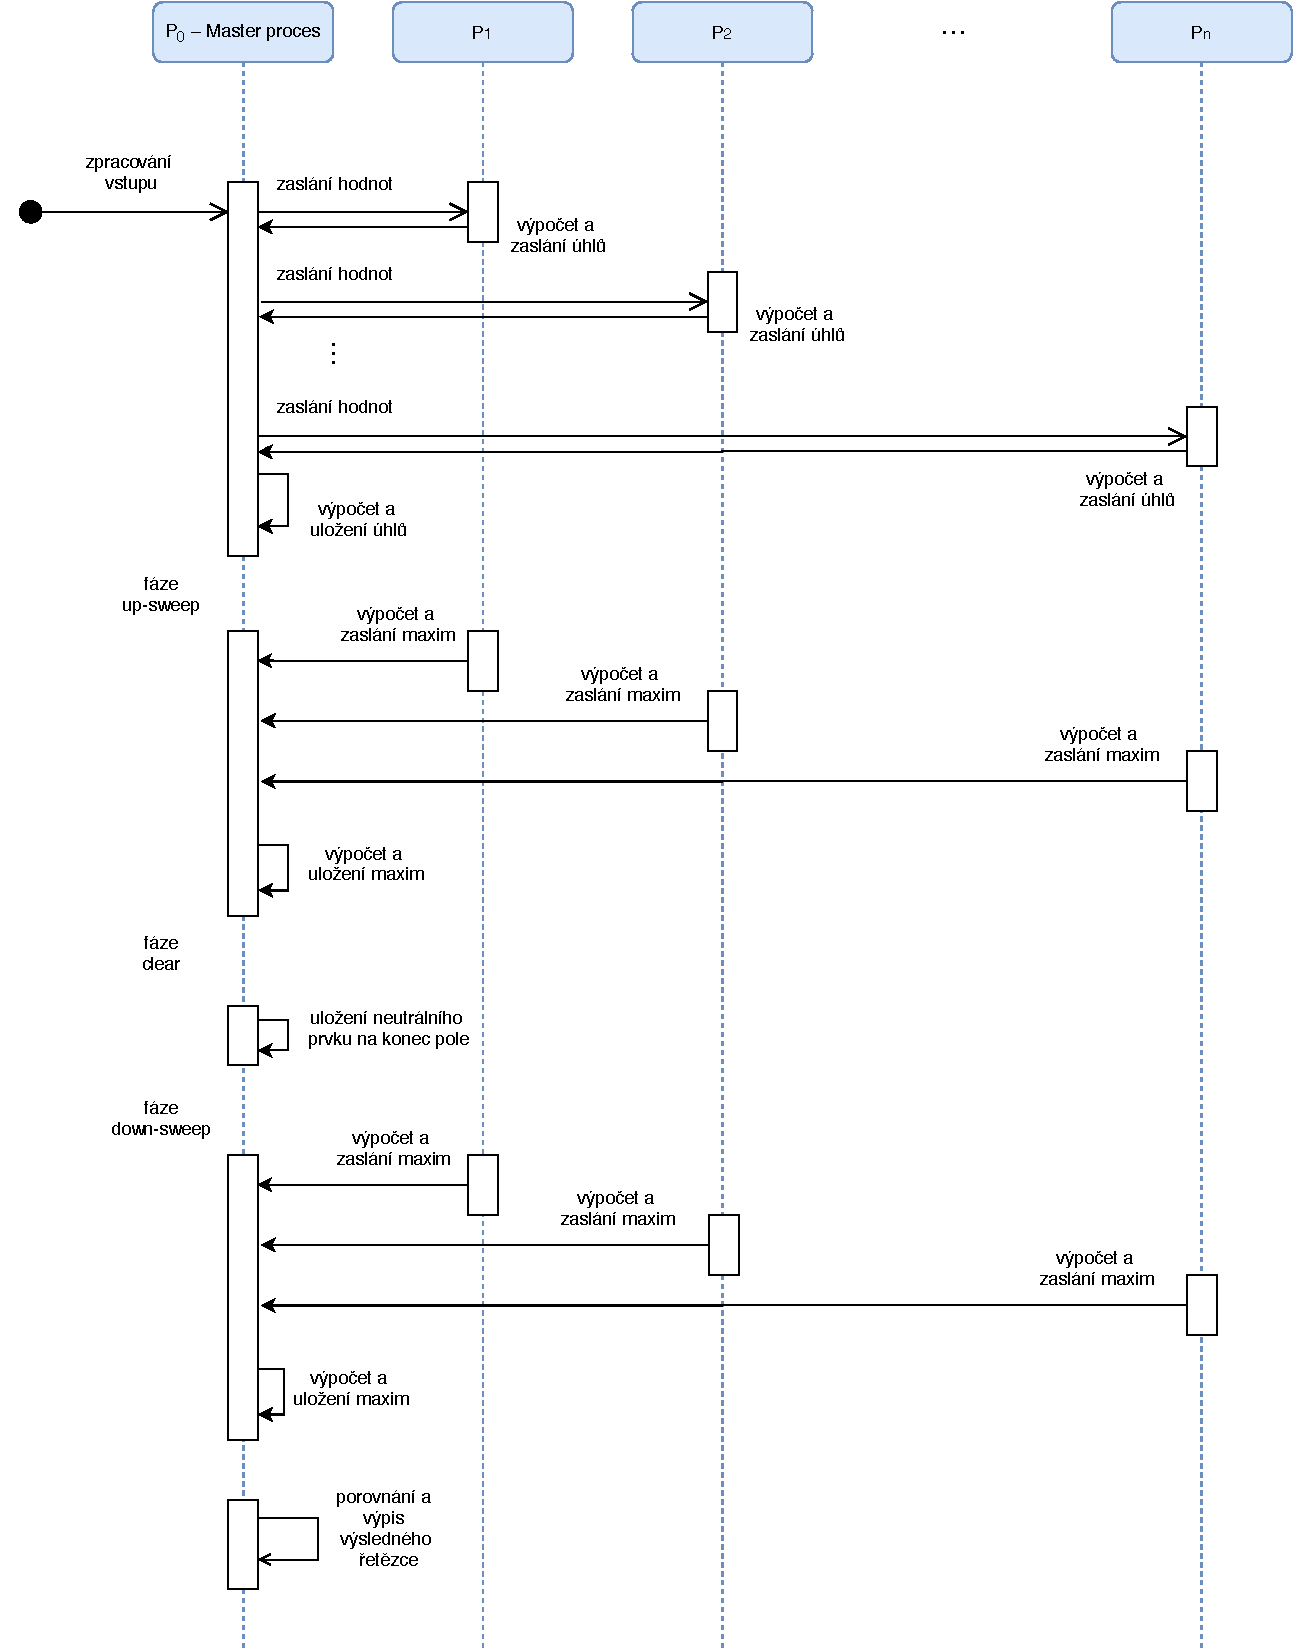
\includegraphics[width=.99\textwidth]{diagram.pdf}
    \caption{Komunikační protokol aplikace zakreslený sekvenčním diagramem.}
\end{figure}

%%%%%%%%%%%%%%%%%%%%%%%%%%%%%%%%%%%%%%%%%%%%%%%%%%%%%%%%%%%%%%%%%%%%%

\section{Experimenty pro ověření časové složitosti}\label{sec:experimenty}

Cílem experimentu bylo ověřit časovou složitost implementace algoritmu
sumy prefixů.
Experimenty byly prováděny na superpočítači Anselm, kde je na jednom
výpočetním uzlu k~dispozici až 16 procesorů.
Proto jsou experimenty prováděny na délkách vstupu do 64, která odpovídá
potřebě 16 procesorů.
Na delších vstupech by výsledky byly zkreslené nedostatkem
fyzických procesorů.
Měřen byl pouze algoritmus sumy prefixů, veškerá režie a další práce
spojená s~kompletním řešením úlohy viditelnosti (parsování hodnot ze vstupu,
inicializace MPI, distribuce hodnot mezi procesy, vypisování, \ldots)
nebyla brána v~potaz.

K~samotnému měření byl využit skriptovací jazyk Python.
Vzhledem k~zaokrouhlování délky vstupu na mocniny 2, se měření provádělo pouze na
vstupech takové délky. (Vstupy jakékoliv jiné délky, se chovají totožně.)
Bylo vygenerováno 32 vstupů o~délkách $1, 2, 4, 8, 16, 32, 64$.
Následně byly seřazeny a $20\%$ nejrychlejších a nejpomalejších hodnot bylo vyřazeno.
Ze zbylých hodnot byly spočítány geometrické průměry a ty byly zaneseny do grafu.

\begin{figure}[H]
    \centering
    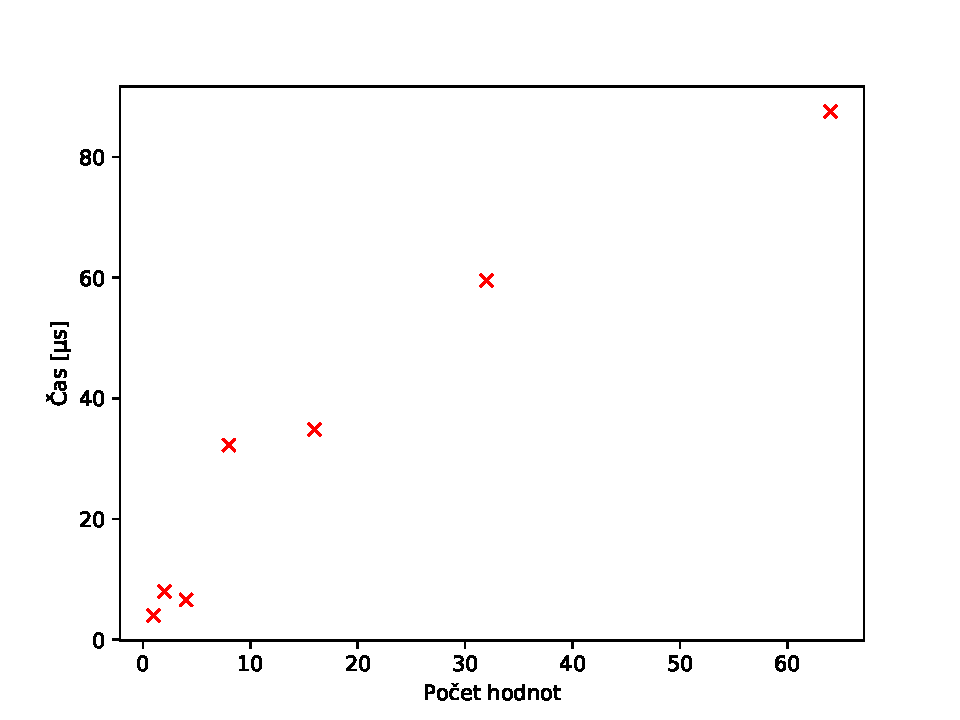
\includegraphics[width=.8\textwidth]{chart.pdf}
    \caption{Délka trvání běhu algoritmu sumy prefixů v~závislosti na délce vstupu.}
\end{figure}

%%%%%%%%%%%%%%%%%%%%%%%%%%%%%%%%%%%%%%%%%%%%%%%%%%%%%%%%%%%%%%%%%%%%%

\section{Závěr}\label{sec:zaver}

Výsledky měření v~kapitole~\ref{sec:experimenty} ukazují, že čas běhu
algorimu sumy prefixů roste logaritmicky s~počtem vstupních hodnot.
Toto zjištění podložené vykonanými experimenty odpovídá odvozené
teoretické časové složitosti v~kapitole~\ref{sec:rozbor}.

%%%%%%%%%%%%%%%%%%%%%%%%%%%%%%%%%%%%%%%%%%%%%%%%%%%%%%%%%%%%%%%%%%%%%

\end{document}
